\documentclass{article}
\usepackage[utf8]{inputenc}
\usepackage{geometry}
\geometry{a4paper, margin=1in}
\usepackage{amsmath}
\usepackage{graphicx}
\usepackage{caption}
\usepackage{lipsum}
\usepackage{biblatex}
\addbibresource{bibliography.bib}

\geometry{a4paper, left=2cm, right=2cm, top=1cm, bottom=2cm}

\begin{document}

\begin{minipage}{0.7\textwidth}
    \small \textbf{Fenómenos Colectivos}  \\
    \small {Facultad de Ciencias, Universidad Nacional Autónoma de México} \\
    \small {Profesora: Dra. Catalina Elizabeth Stern Forgach} \\
    \small {Ayudante: M. Tyra Delgadillo Mendoza} \\
    \small {Fecha de entrega: Viernes 5 de abril del 2024} \\
    \small {Nombre completo: Andrés López González} \\
    \small {La Discusión sobre la Constitución de la Materia en la Época de Boltzmann}
\end{minipage}
\hfill
\begin{minipage}{0.12\textwidth}
    
\includegraphics[width=\linewidth]{logo_universidad}
\end{minipage}\\\\
En sistemas así de microscópicos la fuerza gravitacional pasa totalmente desapercibida en contraste con la fuerza eléctrica producida por las dos partículas de menor carga posible (e). Ahora bien, imaginemos un sistema más usual en la que se usan mucho más partículas y de mayor carga, la fuerza gravitacional será despreciable en un orden increíblemente alto.\\
\section*{Abstract}
La discusión sobre la constitución de la materia durante la época de Ludwig Boltzmann fue un tema central en el desarrollo de la física y la química. En este período, surgieron dos corrientes de pensamiento principales: aquellos que defendían la existencia de una estructura atómica en la materia, y aquellos que sostenían que solo los campos eran importantes, considerando los átomos como una construcción útil pero no necesaria. Este ensayo explora en detalle estas dos perspectivas y sus implicaciones en el contexto histórico y científico de la época.

\subsubsection*{La Perspectiva Atomista}
La perspectiva atomista, defendida por figuras prominentes como Boltzmann, Thomson y Einstein, postulaba que la materia estaba compuesta por partículas fundamentales indivisibles, los átomos. Esta teoría tenía sus raíces en las ideas de los antiguos filósofos griegos, pero fue desarrollada y respaldada por evidencia experimental en el siglo XIX. 

Uno de los principales argumentos a favor del atomismo era la explicación que ofrecía sobre fenómenos macroscópicos como la ley de los gases ideales y la ley de conservación de la masa. Además, la teoría atomista proporcionaba una base sólida para entender fenómenos termodinámicos y la naturaleza de la materia en diferentes estados.

\subsubsection*{Contribuciones de Ludwig Boltzmann}
Ludwig Boltzmann, en particular, desempeñó un papel crucial en la promoción del atomismo y en el desarrollo de la mecánica estadística. Su trabajo en la teoría cinética de los gases y en la derivación de la ecuación de distribución de Maxwell-Boltzmann fue fundamental para establecer la base teórica del atomismo.

Boltzmann también fue pionero en la introducción del concepto de entropía como medida de la probabilidad estadística de un estado en un sistema físico. Esta idea revolucionaria ayudó a unificar la mecánica estadística con la termodinámica, proporcionando una comprensión más profunda de los procesos irreversibles y la segunda ley de la termodinámica.

\begin{figure}[h]
    \centering
    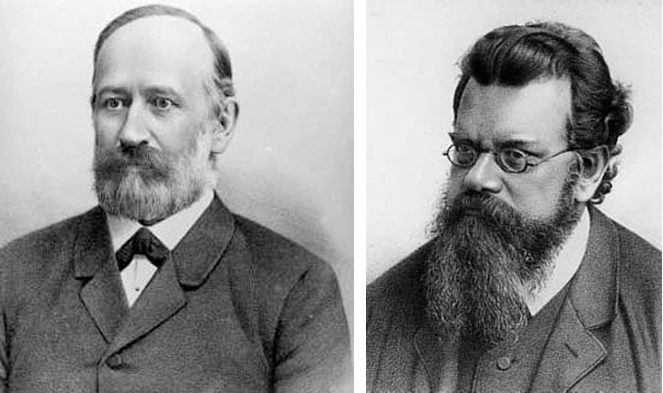
\includegraphics[width=0.5\linewidth]{Boltzmann.png}
    \caption{Ludwig Boltzmann}
    \label{fig:enter-label}
\end{figure}\\

\subsubsection*{La Perspectiva Campo-Céntrica}
Por otro lado, la perspectiva campo-céntrica argumentaba que los campos físicos, como el electromagnético, eran la realidad fundamental, mientras que los átomos eran simplemente una construcción conveniente para explicar ciertos fenómenos. Esta visión fue apoyada por físicos prominentes como James Clerk Maxwell y Oliver Lodge.

La teoría de los campos ofrecía una descripción unificada de fenómenos electromagnéticos, y su éxito en predecir y explicar una amplia gama de fenómenos naturales llevó a muchos científicos a creer que los átomos no eran necesarios para comprender la naturaleza de la materia.

\subsubsection*{Maxwell y la Electrodinámica}
James Clerk Maxwell fue uno de los principales defensores de la perspectiva campo-céntrica. Su teoría de la electrodinámica, expresada en las ecuaciones de Maxwell, proporcionó una descripción completa de los fenómenos electromagnéticos en términos de campos eléctricos y magnéticos.

La teoría de Maxwell tenía una elegancia matemática y una capacidad predictiva que la hacía muy atractiva para muchos científicos de la época. Además, la propagación de las ondas electromagnéticas, predicha por las ecuaciones de Maxwell, ofrecía una explicación convincente de fenómenos como la luz y las ondas de radio sin recurrir a la noción de átomos.

\section*{Conclusión}
La discusión sobre la constitución de la materia en la época de Boltzmann fue un debate fundamental que influyó en el desarrollo posterior de la física y la química. Si bien la perspectiva atomista ganó terreno con el tiempo y se convirtió en la visión predominante en la ciencia moderna, la perspectiva campo-céntrica también dejó un legado duradero en áreas como la física de partículas y la teoría cuántica de campos.

En última instancia, tanto el atomismo como la teoría de los campos han contribuido significativamente a nuestra comprensión de la naturaleza de la materia y el universo en su conjunto, demostrando la riqueza y la complejidad de la exploración científica.

\begin{figure}[h]
    \centering
    
\includegraphics[width=0.5\linewidth]{Atom.png}
    \caption{Representación del átomo}
    \label{fig:enter-label}
\end{figure}\\
\nocite{*}
\printbibliography[title={Bibliografía}]

\end{document}
